\definecolor{opt}{HTML}{51B824}
\definecolor{amm}{HTML}{CC0000}

\section{Cruscotto di valutazione della qualità}
\subsection{Qualità del processo di fornitura}
\subsubsection{1M-PV - Planned value e 2M-EV - Earned value}
%--------- GRAFICO -----------%
\begin{figure*}[!h]
    \centering
    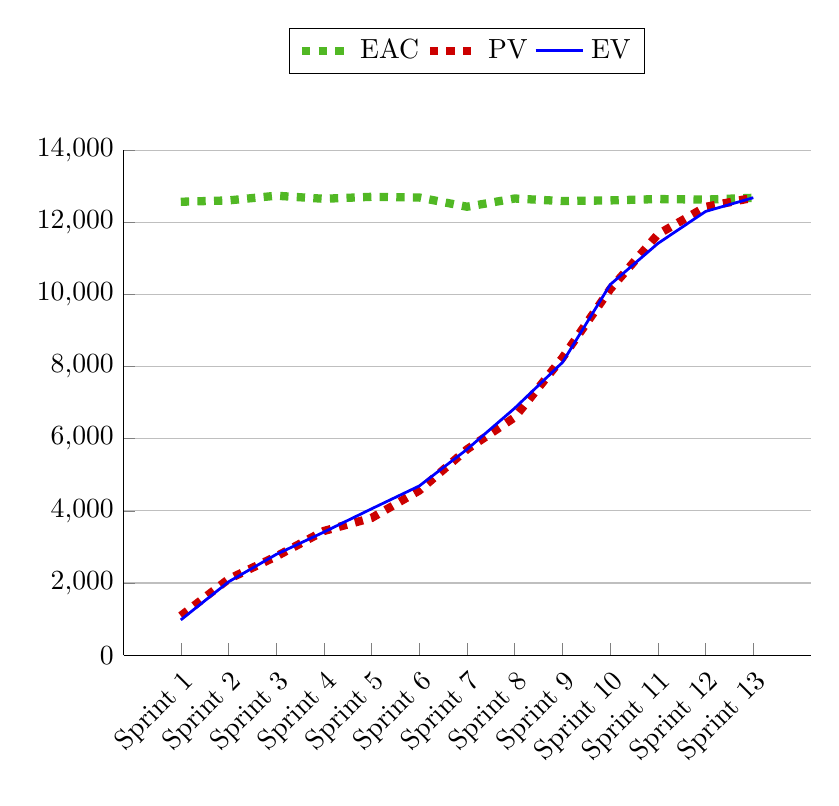
\begin{tikzpicture}
        \begin{axis}[
            width  = 0.85*\textwidth,
            height = 8cm,
            ymajorgrids = true,
            symbolic x coords={Sprint 1, Sprint 2, Sprint 3, Sprint 4, Sprint 5, Sprint 6, Sprint 7, Sprint 8, Sprint 9, Sprint 10, Sprint 11, Sprint 12, Sprint 13},
            xtick = data,
            ymin=0,
            axis lines*=left,
            legend cell align=left,
            legend style={
                at={(0.5,1.15)},
                anchor=south,
                column sep=0.1ex,
                legend columns=3
            },
            xticklabel style={rotate=45, anchor=north east, yshift=0ex, xshift=0ex},
            scaled y ticks = false,
            yticklabel style={/pgf/number format/fixed}
        ]
            \addplot[color=opt, style={dashed, line width=3pt}, mark=none] coordinates { % EAC
                (Sprint 1, 12567.5)
                (Sprint 2, 12605)
                (Sprint 3, 12735)
                (Sprint 4, 12650)
                (Sprint 5, 12705)
                (Sprint 6, 12685)
                (Sprint 7, 12430)
                (Sprint 8, 12657.5)
                (Sprint 9, 12587.5)
                (Sprint 10, 12605)
                (Sprint 11, 12642.5)
                (Sprint 12, 12627.5)
                (Sprint 13, 12677.5)
            };
            \addplot[color=amm, style={dashed, line width=3pt}, mark=none] coordinates { % PV
                (Sprint 1, 1090)
                (Sprint 2, 2107.5)
                (Sprint 3, 2737.5)
                (Sprint 4, 3442.5)
                (Sprint 5, 3804)
                (Sprint 6, 4564.8)
                (Sprint 7, 5706)
                (Sprint 8, 6593.6)
                (Sprint 9, 8242)
                (Sprint 10, 10144)
                (Sprint 11, 11665.6)
                (Sprint 12, 12426.4)
                (Sprint 13, 12680)
            };
            \addplot[color=blue, style={line width=1pt}, mark=none] coordinates { % EV
                (Sprint 1, 977.5)
                (Sprint 2, 2032.5)
                (Sprint 3, 2792.5)
                (Sprint 4, 3412.5)
                (Sprint 5, 4057.6)
                (Sprint 6, 4691.6)
                (Sprint 7, 5706)
                (Sprint 8, 6847.2)
                (Sprint 9, 8115.2)
                (Sprint 10, 10270.8)
                (Sprint 11, 11412)
                (Sprint 12, 12299.6)
                (Sprint 13, 12680)
            };
            \legend{EAC, PV, EV}
        \end{axis}
    \end{tikzpicture}
    \caption{Proiezione del PV e dell'EV}
\end{figure*}
%--------- FINE GRAFICO -----------%

\begin{flushleft}
\textbf{RTB} \\
Visionando il grafico si può notare che i valori di EV e PV quasi si sovrappongono, questo indica la buona riuscita della pianificazione delle attività da parte del gruppo \textit{7Last}. \\
\textbf{PB} \\
Dal grafico completo si evince che il gruppo ha svolto le attività in modo efficiente, con un'evoluzione costante e in linea con la pianificazione. Questo è supportato dal fatto che i valori di EV e PV sono molto vicini tra loro, indicando che il gruppo ha pianificato correttamente le attività, confermando l'andamento positivo del progetto.
\end{flushleft}
    
\newpage
\subsubsection{3M-AC - Actual cost  e 9M-ETC - Estimate to complete}
%--------- GRAFICO -----------%
\begin{figure*}[!h]
    \centering
    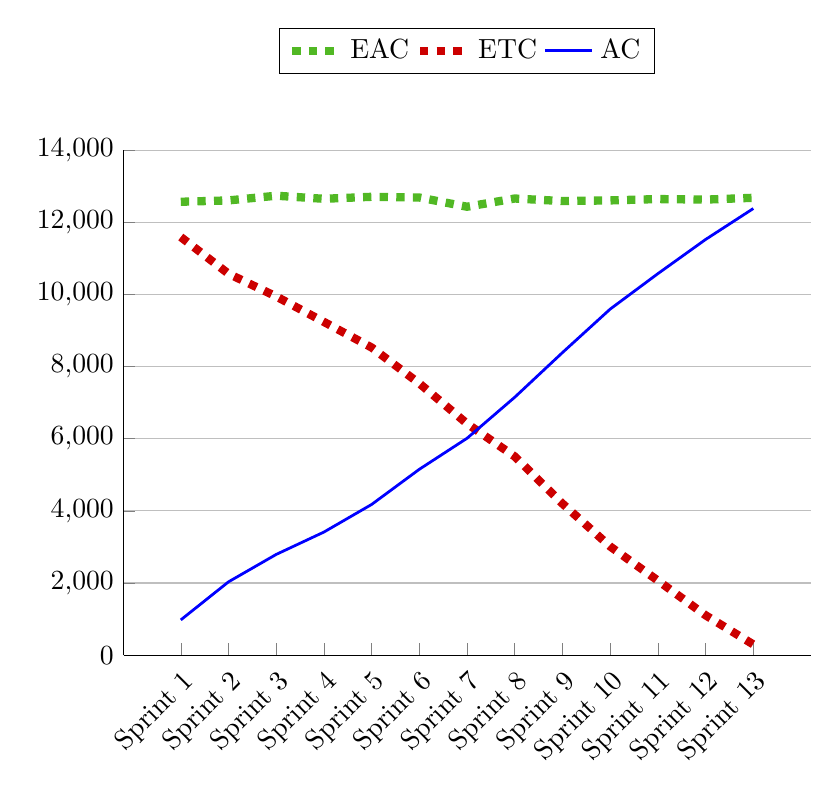
\begin{tikzpicture}
        \begin{axis}[
            width  = 0.85*\textwidth,
            height = 8cm,
            ymajorgrids = true,
            symbolic x coords={Sprint 1, Sprint 2, Sprint 3, Sprint 4, Sprint 5, Sprint 6, Sprint 7, Sprint 8, Sprint 9, Sprint 10, Sprint 11, Sprint 12, Sprint 13},
            xtick = data,
            ymin=0,
            axis lines*=left,
            legend cell align=left,
            legend style={
                at={(0.5,1.15)},
                anchor=south,
                column sep=0.1ex,
                legend columns=3
            },
            xticklabel style={rotate=45, anchor=north east, yshift=0ex, xshift=0ex},
            scaled y ticks = false,
            yticklabel style={/pgf/number format/fixed}
        ]
            \addplot[color=opt, style={dashed, line width=3pt}, mark=none] coordinates { % EAC
                (Sprint 1, 12567.5)
                (Sprint 2, 12605)
                (Sprint 3, 12735)
                (Sprint 4, 12650)
                (Sprint 5, 12705)
                (Sprint 6, 12685)
                (Sprint 7, 12430)
                (Sprint 8, 12657.5)
                (Sprint 9, 12587.5)
                (Sprint 10, 12605)
                (Sprint 11, 12642.5)
                (Sprint 12, 12627.5)
                (Sprint 13, 12677.5)
            };
            \addplot[color=amm, style={dashed, line width=3pt}, mark=none] coordinates { % ETC
                (Sprint 1, 11590)
                (Sprint 2, 10572.5)
                (Sprint 3, 9942.5)
                (Sprint 4, 9237.5)
                (Sprint 5, 8527.5)
                (Sprint 6, 7532.5)
                (Sprint 7, 6417.5)
                (Sprint 8, 5507.5)
                (Sprint 9, 4200)
                (Sprint 10, 3012.5)
                (Sprint 11, 2067.5)
                (Sprint 12, 1105)
                (Sprint 13, 297.5)
            };
            \addplot[color=blue, style={line width=1pt}, mark=none] coordinates { % AC
                (Sprint 1, 977.5)
                (Sprint 2, 2032.5)
                (Sprint 3, 2792.5)
                (Sprint 4, 3412.5)
                (Sprint 5, 4177.5)
                (Sprint 6, 5152.5)
                (Sprint 7, 6012.5)
                (Sprint 8, 7150)
                (Sprint 9, 8387.5)
                (Sprint 10, 9592.5)
                (Sprint 11, 10575)
                (Sprint 12, 11522.5)
                (Sprint 13, 12380)
            };
            \legend{EAC, ETC, AC}
        \end{axis}
    \end{tikzpicture}
    \caption{Proiezione dell'AC e dell'ETC}
\end{figure*}
%--------- FINE GRAFICO -----------%

\begin{flushleft}
\textbf{RTB} \\
Il grafico evidenzia chiaramente un aumento progressivo dei costi (AC). Parallelamente, si osserva una diminuzione della stima dei costi a finire (ETC), che sta calando in modo proporzionale all'incremento dei costi. \\
\textbf{PB} \\
In questo secondo periodo viene confermato l'andamento evidenziato in quello precedente, con i costi reali (AC) che aumentano in modo proporzionale alla diminuzione della stima dei costi a finire (ETC). Questo indica che il gruppo ha svolto le attività in modo efficiente, con un allineamento tra i costi reali e quelli preventivati.
\end{flushleft}

\newpage
\subsubsection{4M-SV - Schedule variance e 5M-CV - Cost variance}
%--------- GRAFICO -----------%
\begin{figure*}[!h]
    \centering
    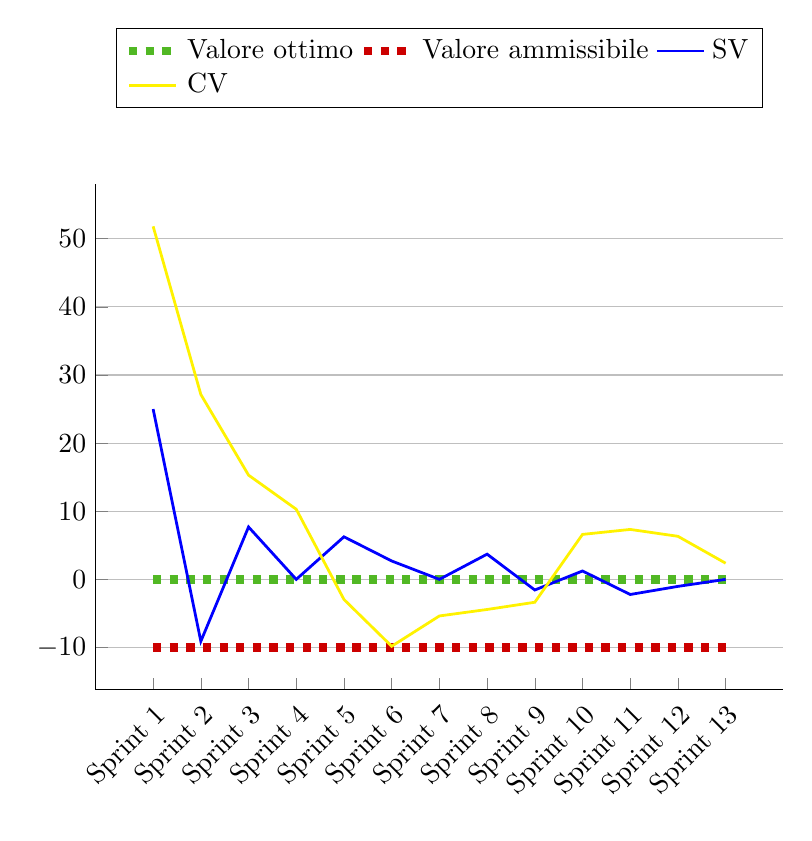
\begin{tikzpicture}
        \begin{axis}[
            width  = 0.85*\textwidth,
            height = 8cm,
            ymajorgrids = true,
            symbolic x coords={Sprint 1, Sprint 2, Sprint 3, Sprint 4, Sprint 5, Sprint 6, Sprint 7, Sprint 8, Sprint 9, Sprint 10, Sprint 11, Sprint 12, Sprint 13},
            xtick = data,
            axis lines*=left,
            legend cell align=left,
            legend style={
                at={(0.5,1.15)},
                anchor=south,
                column sep=0.1ex,
                legend columns=3
            },
            xticklabel style={rotate=45, anchor=north east, yshift=0ex, xshift=0ex}
        ]
            \addplot[color=opt, style={dashed, line width=3pt}, mark=none] coordinates { % ottimo = 0
                (Sprint 1, 0)
                (Sprint 2, 0)
                (Sprint 3, 0)
                (Sprint 4, 0)
                (Sprint 5, 0)
                (Sprint 6, 0)
                (Sprint 7, 0)
                (Sprint 8, 0)
                (Sprint 9, 0)
                (Sprint 10, 0)
                (Sprint 11, 0)
                (Sprint 12, 0)
                (Sprint 13, 0)
            };
            \addplot[color=amm, style={dashed, line width=3pt}, mark=none] coordinates { % ammissibile = -10
                (Sprint 1, -10)
                (Sprint 2, -10)
                (Sprint 3, -10)
                (Sprint 4, -10)
                (Sprint 5, -10)
                (Sprint 6, -10)
                (Sprint 7, -10)
                (Sprint 8, -10)
                (Sprint 9, -10)
                (Sprint 10, -10)
                (Sprint 11, -10)
                (Sprint 12, -10)
                (Sprint 13, -10)
            };
            \addplot[color=blue, style={line width=1pt}, mark=none] coordinates { % SV
                (Sprint 1, 25)
                (Sprint 2, -9.09)
                (Sprint 3, 7.69)
                (Sprint 4, 0)
                (Sprint 5, 6.25)
                (Sprint 6, 2.7)
                (Sprint 7, 0)
                (Sprint 8, 3.7)
                (Sprint 9, -1.56)
                (Sprint 10, 1.23)
                (Sprint 11, -2.22)
                (Sprint 12, -1.03)
                (Sprint 13, 0)
            };
            \addplot[color=yellow, style={line width=1pt}, mark=none] coordinates { % CV
                (Sprint 1, 51.82)
                (Sprint 2, 27.14)
                (Sprint 3, 15.30)
                (Sprint 4, 10.29)
                (Sprint 5, -2.95)
                (Sprint 6, -9.82)
                (Sprint 7, -5.37)
                (Sprint 8, -4.42)
                (Sprint 9, -3.36)
                (Sprint 10, 6.6)
                (Sprint 11, 7.33)
                (Sprint 12, 6.32)
                (Sprint 13, 2.37)
            };
            \legend{Valore ottimo, Valore ammissibile, SV, CV}
        \end{axis}
    \end{tikzpicture}
    \caption{Andamento percentuale di SV e CV}
\end{figure*}
%--------- FINE GRAFICO -----------%
\begin{flushleft}
\textbf{RTB} \\
Dal grafico si nota come sia SV che CV siano inizialmente elevati, per poi decrescere durante la prosecuzione del progetto, in particolare si nota un andamento altalenante del SV. L'andamento inizialmente alto del Schedule Variance (SV) e del Cost Variance (CV) indica una possibile sovrastima iniziale dei tempi e dei costi, dovuta all'inesperienza del team. La variabilità del SV suggerisce che le stime di tempistiche iniziali erano eccessivamente conservative, con aggiustamenti successivi man mano che il team acquisiva esperienza. La decrescita nel tempo di entrambe le metriche mostra che il gruppo sta diventando più preciso nelle sue previsioni, con un allineamento progressivo dei costi e delle tempistiche reali rispetto a quelle pianificate. \\
\textbf{PB} \\
L'andamento del grafico nella seconda parte del progetto conferma il trend positivo iniziato nel periodo precedente, con SV e CV che si avvicinano ai valori ottimali.
\end{flushleft}

\newpage
\subsubsection{8M-EAC - Estimated at completion}
%--------- GRAFICO -----------%
\begin{figure*}[!h]
    \centering
    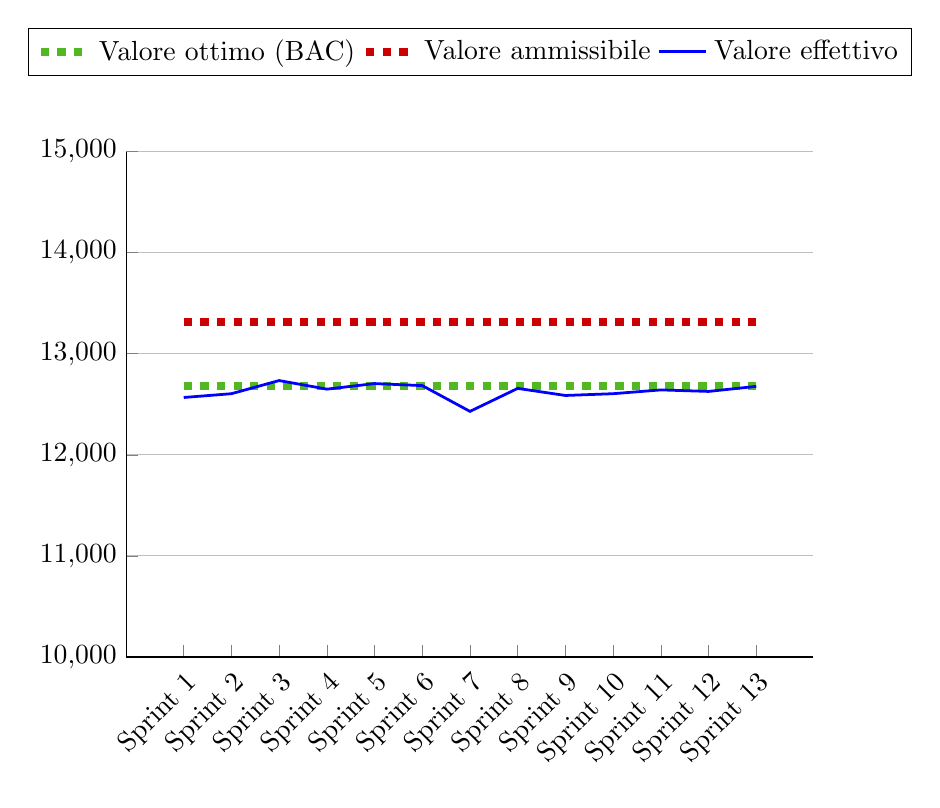
\begin{tikzpicture}
        \begin{axis}[
            width  = 0.85*\textwidth,
            height = 8cm,
            ymajorgrids = true,
            symbolic x coords={Sprint 1, Sprint 2, Sprint 3, Sprint 4, Sprint 5, Sprint 6, Sprint 7, Sprint 8, Sprint 9, Sprint 10, Sprint 11, Sprint 12, Sprint 13},
            xtick = data,
            ytick = {10000, 11000, 12000, 13000, 14000, 15000},
            ymin=10000, ymax=15000,
            axis lines*=left,
            legend cell align=left,
            legend style={
                at={(0.5,1.15)},
                anchor=south,
                column sep=0.1ex,
                legend columns=3
            },
            xticklabel style={rotate=45, anchor=north east, yshift=0ex, xshift=0ex},
            scaled y ticks = false,
            yticklabel style={/pgf/number format/fixed}
        ]
            \addplot[color=opt, style={dashed, line width=3pt}, mark=none] coordinates { % ottimo = BAC
                (Sprint 1, 12680)
                (Sprint 2, 12680)
                (Sprint 3, 12680)
                (Sprint 4, 12680)
                (Sprint 5, 12680)
                (Sprint 6, 12680)
                (Sprint 7, 12680)
                (Sprint 8, 12680)
                (Sprint 9, 12680)
                (Sprint 10, 12680)
                (Sprint 11, 12680)
                (Sprint 12, 12680)
                (Sprint 13, 12680)
            };
            \addplot[color=amm, style={dashed, line width=3pt}, mark=none] coordinates { % ammissibile = BAC + 5%
                (Sprint 1, 13314)
                (Sprint 2, 13314)
                (Sprint 3, 13314)
                (Sprint 4, 13314)
                (Sprint 5, 13314)
                (Sprint 6, 13314)
                (Sprint 7, 13314)
                (Sprint 8, 13314)
                (Sprint 9, 13314)
                (Sprint 10, 13314)
                (Sprint 11, 13314)
                (Sprint 12, 13314)
                (Sprint 13, 13314)
            };
            \addplot[color=blue, style={line width=1pt}, mark=none] coordinates { % EAC
                (Sprint 1, 12567.5)
                (Sprint 2, 12605)
                (Sprint 3, 12735)
                (Sprint 4, 12650)
                (Sprint 5, 12705)
                (Sprint 6, 12685)
                (Sprint 7, 12430)
                (Sprint 8, 12657.5)
                (Sprint 9, 12587.5)
                (Sprint 10, 12605)
                (Sprint 11, 12642.5)
                (Sprint 12, 12627.5)
                (Sprint 13, 12677.5)
            };
            \legend{Valore ottimo (BAC), Valore ammissibile, Valore effettivo}
        \end{axis}
    \end{tikzpicture}
    \caption{Proiezione dell'EAC}
\end{figure*}
%--------- FINE GRAFICO -----------%
\begin{flushleft}
\textbf{RTB} \\
Osservando il grafico si può notare come l'EAC sia quasi sovrapposto al BAC durante i periodi di progetto analizzati fino ad ora. Questa situazione riflette come \textit{7Last} abbia attuato una gestione efficace sia dei costi che delle tempistiche durante i periodi analizzati fino ad ora. \\
\textbf{PB} \\
Anche in questo grafico abbiamo una conferma dell'andamento rilevato nella prima parte del progetto, con l'EAC che si mantiene costantemente vicino al BAC. Questo indica che il gruppo ha svolto le attività in modo efficiente, con un allineamento tra i costi reali e quelli preventivati, senza variazioni significative.
\end{flushleft}

\newpage
\subsection{Qualità del processo di analisi dei requisiti}
\subsubsection{11M-PRO - Percentuale requisiti obbligatori}
%--------- GRAFICO -----------%
\begin{figure*}[!h]
    \centering
    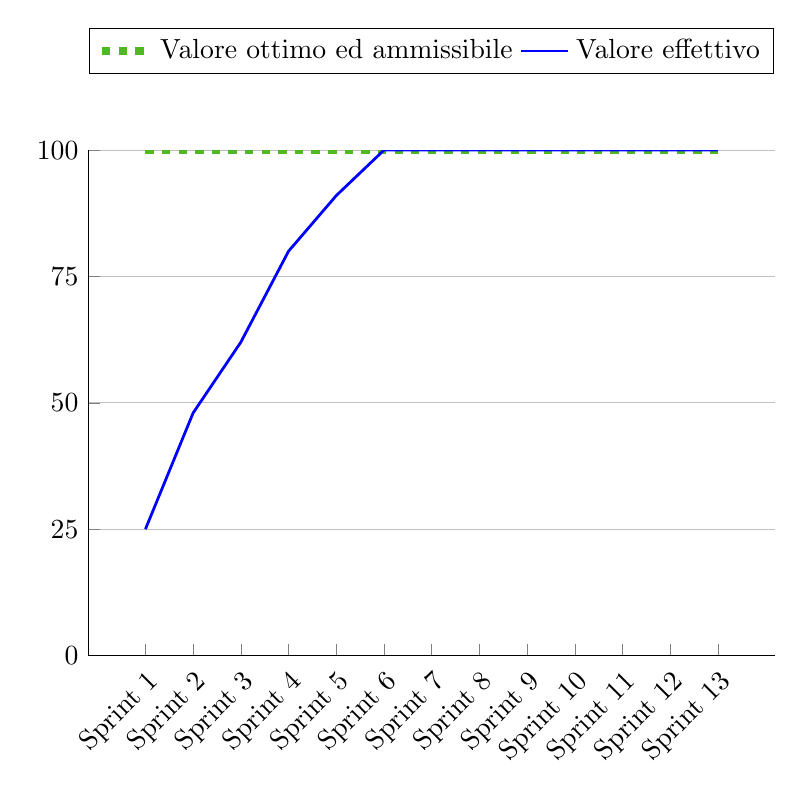
\begin{tikzpicture}
        \begin{axis}[
            width  = 0.85*\textwidth,
            height = 8cm,
            ymajorgrids = true,
            symbolic x coords={Sprint 1, Sprint 2, Sprint 3, Sprint 4, Sprint 5, Sprint 6, Sprint 7, Sprint 8, Sprint 9, Sprint 10, Sprint 11, Sprint 12, Sprint 13},
            xtick = data,
            ytick = {0, 25, 50, 75, 100},
            ymin=0, ymax=100,
            axis lines*=left,
            legend cell align=left,
            legend style={
                at={(0.5,1.15)},
                anchor=south,
                column sep=0.1ex,
                legend columns=3
            },
            xticklabel style={rotate=45, anchor=north east, yshift=0ex, xshift=0ex}
            ]
            \addplot[color=opt, style={dashed, line width=3pt}, mark=none] coordinates { % ottimo = 100
                (Sprint 1, 100)
                (Sprint 2, 100)
                (Sprint 3, 100)
                (Sprint 4, 100)
                (Sprint 5, 100)
                (Sprint 6, 100)
                (Sprint 7, 100)
                (Sprint 8, 100)
                (Sprint 9, 100)
                (Sprint 10, 100)
                (Sprint 11, 100)
                (Sprint 12, 100)
                (Sprint 13, 100)
            };
            \addplot[color=blue, style={line width=1pt}, mark=none] coordinates { % effettivo
                (Sprint 1, 25)
                (Sprint 2, 48)
                (Sprint 3, 62)
                (Sprint 4, 80)
                (Sprint 5, 91)
                (Sprint 6, 100)
                (Sprint 7, 100)
                (Sprint 8, 100)
                (Sprint 9, 100)
                (Sprint 10, 100)
                (Sprint 11, 100)
                (Sprint 12, 100)
                (Sprint 13, 100)
            };
            \legend{Valore ottimo ed ammissibile, Valore effettivo}
        \end{axis}
    \end{tikzpicture}
    \caption{Percentuale di copertura dei requisiti obbligatori}
\end{figure*}
%--------- FINE GRAFICO -----------% \\
\begin{flushleft}
\textbf{PB} \\
Dal grafico si evince come a partire dai primi sprint il gruppo \textit{7Last} abbia lavorato in modo costante per soddisfare i requisiti obbligatori. Questo è confermato dal fatto che la percentuale di requisiti obbligatori soddisfatti è sempre cresciuta, fino al raggiungimento del 100\% già a partire dal sesto sprint, confermando che il gruppo ha lavorato in modo efficace e con un'attenzione costante ai requisiti obbligatori.
\end{flushleft}

\newpage
\subsubsection{12M-PRD - Percentuale requisiti desiderabili}
%--------- GRAFICO -----------%
\begin{figure*}[!h]
    \centering
    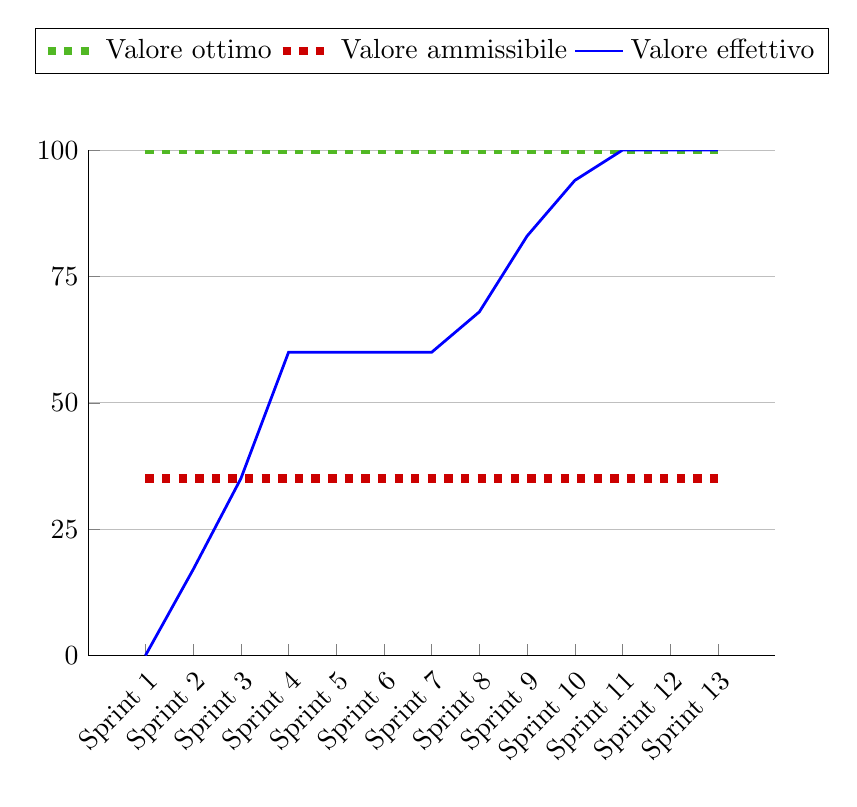
\begin{tikzpicture}
        \begin{axis}[
            width  = 0.85*\textwidth,
            height = 8cm,
            ymajorgrids = true,
            symbolic x coords={Sprint 1, Sprint 2, Sprint 3, Sprint 4, Sprint 5, Sprint 6, Sprint 7, Sprint 8, Sprint 9, Sprint 10, Sprint 11, Sprint 12, Sprint 13},
            xtick = data,
            ytick = {0, 25, 50, 75, 100},
            ymin=0, ymax=100,
            axis lines*=left,
            legend cell align=left,
            legend style={
                at={(0.5,1.15)},
                anchor=south,
                column sep=0.1ex,
                legend columns=3
            },
            xticklabel style={rotate=45, anchor=north east, yshift=0ex, xshift=0ex}
            ]
            \addplot[color=opt, style={dashed, line width=3pt}, mark=none] coordinates { % ottimo = 100
                (Sprint 1, 100)
                (Sprint 2, 100)
                (Sprint 3, 100)
                (Sprint 4, 100)
                (Sprint 5, 100)
                (Sprint 6, 100)
                (Sprint 7, 100)
                (Sprint 8, 100)
                (Sprint 9, 100)
                (Sprint 10, 100)
                (Sprint 11, 100)
                (Sprint 12, 100)
                (Sprint 13, 100)
            };
            \addplot[color=amm, style={dashed, line width=3pt}, mark=none] coordinates { % ammissibile = 35
                (Sprint 1, 35)
                (Sprint 2, 35)
                (Sprint 3, 35)
                (Sprint 4, 35)
                (Sprint 5, 35)
                (Sprint 6, 35)
                (Sprint 7, 35)
                (Sprint 8, 35)
                (Sprint 9, 35)
                (Sprint 10, 35)
                (Sprint 11, 35)
                (Sprint 12, 35)
                (Sprint 13, 35)
            };
            \addplot[color=blue, style={line width=1pt}, mark=none] coordinates { % effettivo
                (Sprint 1, 0)
                (Sprint 2, 17)
                (Sprint 3, 35)
                (Sprint 4, 60)
                (Sprint 5, 60)
                (Sprint 6, 60)
                (Sprint 7, 60)
                (Sprint 8, 68)
                (Sprint 9, 83)
                (Sprint 10, 94)
                (Sprint 11, 100)
                (Sprint 12, 100)
                (Sprint 13, 100)
            };
            \legend{Valore ottimo, Valore ammissibile, Valore effettivo}
        \end{axis}
    \end{tikzpicture}
    \caption{Percentuale di copertura dei requisiti desiderabili}
\end{figure*}
%--------- FINE GRAFICO -----------% \\
\begin{flushleft}
\textbf{PB} \\
Il grafico mostra come il gruppo \textit{7Last} abbia lavorato per soddisfare i requisiti desiderabili, raggiungendo l'ottimo risultato del 100\% di copertura. Questo conferma che il gruppo ha lavorato in modo efficace e con un'attenzione costante ai requisiti desiderabili.
\end{flushleft}

\newpage
\subsubsection{13M-PRO - Percentuale requisiti opzionali}
%--------- GRAFICO -----------%
\begin{figure*}[!h]
    \centering
    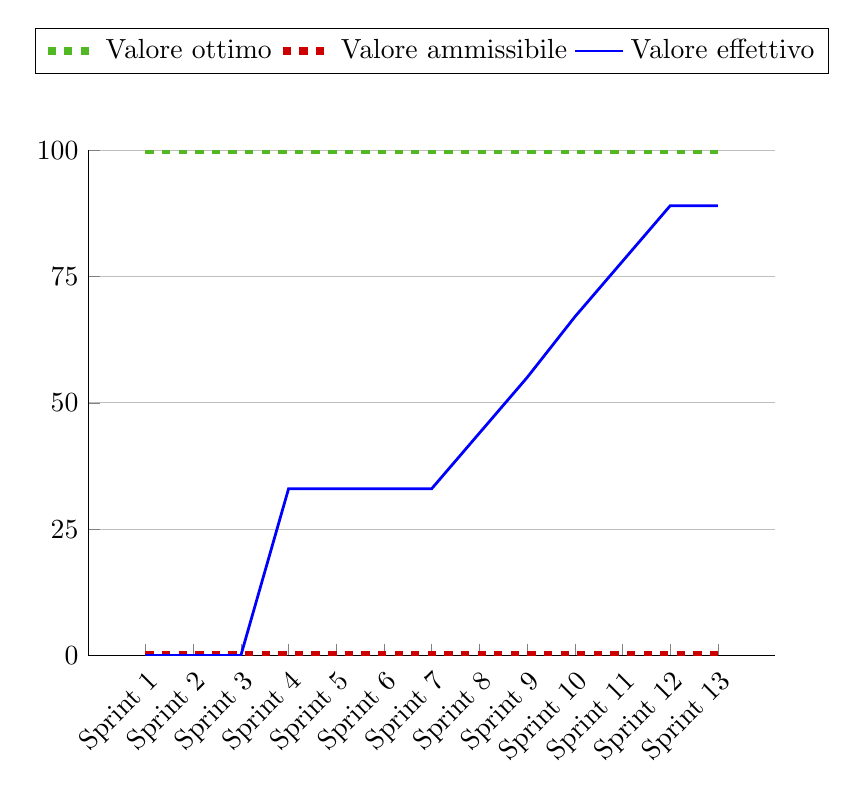
\begin{tikzpicture}
        \begin{axis}[
            width  = 0.85*\textwidth,
            height = 8cm,
            ymajorgrids = true,
            symbolic x coords={Sprint 1, Sprint 2, Sprint 3, Sprint 4, Sprint 5, Sprint 6, Sprint 7, Sprint 8, Sprint 9, Sprint 10, Sprint 11, Sprint 12, Sprint 13},
            xtick = data,
            ytick = {0, 25, 50, 75, 100},
            ymin=0, ymax=100,
            axis lines*=left,
            legend cell align=left,
            legend style={
                at={(0.5,1.15)},
                anchor=south,
                column sep=0.1ex,
                legend columns=3
            },
            xticklabel style={rotate=45, anchor=north east, yshift=0ex, xshift=0ex}
            ]
            \addplot[color=opt, style={dashed, line width=3pt}, mark=none] coordinates { % ottimo = 100
                (Sprint 1, 100)
                (Sprint 2, 100)
                (Sprint 3, 100)
                (Sprint 4, 100)
                (Sprint 5, 100)
                (Sprint 6, 100)
                (Sprint 7, 100)
                (Sprint 8, 100)
                (Sprint 9, 100)
                (Sprint 10, 100)
                (Sprint 11, 100)
                (Sprint 12, 100)
                (Sprint 13, 100)
            };
            \addplot[color=amm, style={dashed, line width=3pt}, mark=none] coordinates { % ammissibile = 0
                (Sprint 1, 0)
                (Sprint 2, 0)
                (Sprint 3, 0)
                (Sprint 4, 0)
                (Sprint 5, 0)
                (Sprint 6, 0)
                (Sprint 7, 0)
                (Sprint 8, 0)
                (Sprint 9, 0)
                (Sprint 10, 0)
                (Sprint 11, 0)
                (Sprint 12, 0)
                (Sprint 13, 0)
            };
            \addplot[color=blue, style={line width=1pt}, mark=none] coordinates { % effettivo
                (Sprint 1, 0)
                (Sprint 2, 0)
                (Sprint 3, 0)
                (Sprint 4, 33)
                (Sprint 5, 33)
                (Sprint 6, 33)
                (Sprint 7, 33)
                (Sprint 8, 44)
                (Sprint 9, 55)
                (Sprint 10, 67)
                (Sprint 11, 78)
                (Sprint 12, 89)
                (Sprint 13, 89)
            };
            \legend{Valore ottimo, Valore ammissibile, Valore effettivo}
        \end{axis}
    \end{tikzpicture}
    \caption{Percentuale di copertura dei requisiti opzionali}
\end{figure*}
%--------- FINE GRAFICO -----------% \\
\begin{flushleft}
\textbf{PB} \\
Il grafico mostra come il gruppo \textit{7Last} abbia lavorato per soddisfare i requisiti opzionali, con una crescita quasi costante della percentuale di requisiti soddisfatti. Questo conferma che il gruppo ha lavorato in modo efficace. 
\end{flushleft}

\newpage
\subsection{Qualità del processo di documentazione}
\subsubsection{19M-IG - Indice di Gulpease}
%--------- GRAFICO -----------%
\begin{figure*}[!h]
    \centering
    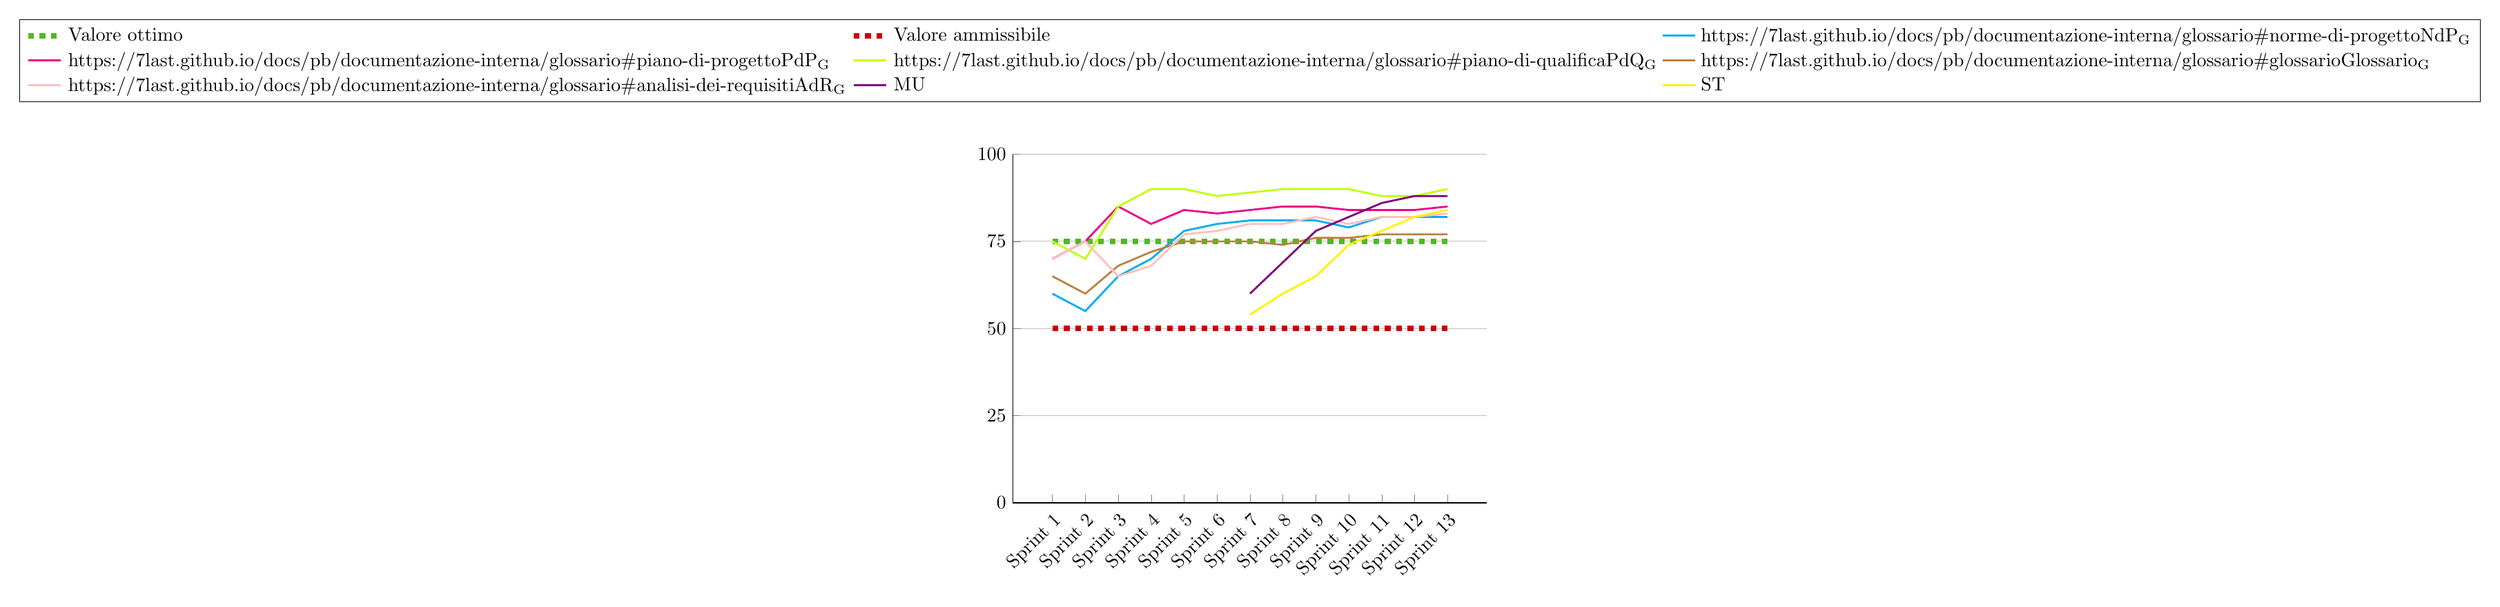
\begin{tikzpicture}
        \begin{axis}[
            width  = 0.85*\textwidth,
            height = 8cm,
            ymajorgrids = true,
            symbolic x coords={Sprint 1, Sprint 2, Sprint 3, Sprint 4, Sprint 5, Sprint 6, Sprint 7, Sprint 8, Sprint 9, Sprint 10, Sprint 11, Sprint 12, Sprint 13},
            xtick = data,
            ytick = {0, 25, 50, 75, 100},
            ymin=0, ymax=100,
            axis lines*=left,
            legend cell align=left,
            legend style={
                at={(0.5,1.15)},
                anchor=south,
                column sep=0.1ex,
                legend columns=3
            },
            xticklabel style={rotate=45, anchor=north east, yshift=0ex, xshift=0ex}
        ]
            \addplot[color=opt, style={dashed, line width=3pt}, mark=none] coordinates { % ottimo = 75
                (Sprint 1, 75)
                (Sprint 2, 75)
                (Sprint 3, 75)
                (Sprint 4, 75)
                (Sprint 5, 75)
                (Sprint 6, 75)
                (Sprint 7, 75)
                (Sprint 8, 75)
                (Sprint 9, 75)
                (Sprint 10, 75)
                (Sprint 11, 75)
                (Sprint 12, 75)
                (Sprint 13, 75)
            };
            \addplot[color=amm, style={dashed, line width=3pt}, mark=none] coordinates { % ammissibile = 50
                (Sprint 1, 50)
                (Sprint 2, 50)
                (Sprint 3, 50)
                (Sprint 4, 50)
                (Sprint 5, 50)
                (Sprint 6, 50)
                (Sprint 7, 50)
                (Sprint 8, 50)
                (Sprint 9, 50)
                (Sprint 10, 50)
                (Sprint 11, 50)
                (Sprint 12, 50)
                (Sprint 13, 50)
            };
            \addplot[color=cyan, style={line width=1pt}, mark=none] coordinates { % norme di progetto
                (Sprint 1, 60)
                (Sprint 2, 55)
                (Sprint 3, 65)
                (Sprint 4, 70)
                (Sprint 5, 78)
                (Sprint 6, 80)
                (Sprint 7, 81)
                (Sprint 8, 81)
                (Sprint 9, 81)
                (Sprint 10, 79)
                (Sprint 11, 82)
                (Sprint 12, 82)
                (Sprint 13, 82)
            };
            \addplot[color=magenta, style={line width=1pt}, mark=none] coordinates { % piano di progetto
                (Sprint 1, 70)
                (Sprint 2, 75)
                (Sprint 3, 85)
                (Sprint 4, 80)
                (Sprint 5, 84)
                (Sprint 6, 83)
                (Sprint 7, 84)
                (Sprint 8, 85)
                (Sprint 9, 85)
                (Sprint 10, 84)
                (Sprint 11, 84)
                (Sprint 12, 84)
                (Sprint 13, 85)
            };
            \addplot[color=lime, style={line width=1pt}, mark=none] coordinates { % piano di qualifica
                (Sprint 1, 75)
                (Sprint 2, 70)
                (Sprint 3, 85)
                (Sprint 4, 90)
                (Sprint 5, 90)
                (Sprint 6, 88)
                (Sprint 7, 89)
                (Sprint 8, 90)
                (Sprint 9, 90)
                (Sprint 10, 90)
                (Sprint 11, 88)
                (Sprint 12, 88)
                (Sprint 13, 90)
            };
            \addplot[color=brown, style={line width=1pt}, mark=none] coordinates { % glossario
                (Sprint 1, 65)
                (Sprint 2, 60)
                (Sprint 3, 68)
                (Sprint 4, 72)
                (Sprint 5, 75)
                (Sprint 6, 75)
                (Sprint 7, 75)
                (Sprint 8, 74)
                (Sprint 9, 76)
                (Sprint 10, 76)
                (Sprint 11, 77)
                (Sprint 12, 77)
                (Sprint 13, 77)
            };
            \addplot[color=pink, style={line width=1pt}, mark=none] coordinates { % analisi dei requisiti
                (Sprint 1, 70)
                (Sprint 2, 75)
                (Sprint 3, 65)
                (Sprint 4, 68)
                (Sprint 5, 77)
                (Sprint 6, 78)
                (Sprint 7, 80)
                (Sprint 8, 80)
                (Sprint 9, 82)
                (Sprint 10, 80)
                (Sprint 11, 82)
                (Sprint 12, 82)
                (Sprint 13, 83)
            };
            \addplot[color=violet, style={line width=1pt}, mark=none] coordinates { % manuale utente
                (Sprint 7, 60)
                (Sprint 8, 69)
                (Sprint 9, 78)
                (Sprint 10, 82)
                (Sprint 11, 86)
                (Sprint 12, 88)
                (Sprint 13, 88)
            };
            \addplot[color=yellow, style={line width=1pt}, mark=none] coordinates { % specifica tecnica
                (Sprint 7, 54)
                (Sprint 8, 60)
                (Sprint 9, 65)
                (Sprint 10, 74)
                (Sprint 11, 78)
                (Sprint 12, 82)
                (Sprint 13, 84)
            };
            \legend{Valore ottimo, Valore ammissibile, \href{https://7last.github.io/docs/pb/documentazione-interna/glossario\#norme-di-progetto}{NdP\textsubscript{G}}, \href{https://7last.github.io/docs/pb/documentazione-interna/glossario\#piano-di-progetto}{PdP\textsubscript{G}}, \href{https://7last.github.io/docs/pb/documentazione-interna/glossario\#piano-di-qualifica}{PdQ\textsubscript{G}}, \href{https://7last.github.io/docs/pb/documentazione-interna/glossario\#glossario}{Glossario\textsubscript{G}}, \href{https://7last.github.io/docs/pb/documentazione-interna/glossario\#analisi-dei-requisiti}{AdR\textsubscript{G}}, MU, ST}
        \end{axis}
    \end{tikzpicture}
    \caption{Andamento indice di Gulpease per ciascun documento}
\end{figure*}
%--------- FINE GRAFICO -----------%
\begin{flushleft}
\textbf{RTB} \\
Visionando il grafico si può notare una tendenza generale di crescita, eccetto per alcuni documenti. L'indice relativamente basso rispetto agli altri documenti rappresenta il \href{https://7last.github.io/docs/pb/documentazione-interna/glossario\#glossario}{glossario\textsubscript{G}}, il quale contiene descrizioni di natura tecnica che possono influire negativamente sull'indice di Gulpease. \\
\textbf{PB} \\
Il grafico mostra come la qualità della documentazione prodotta verso la fine del progetto sia sempre sopra il valore ottimo prestabilito, con un andamento generale di crescita. 
\end{flushleft}

\newpage
\subsubsection{20M-CO - Correttezza ortografica}
%--------- GRAFICO -----------%
\begin{figure*}[!h]
    \centering
    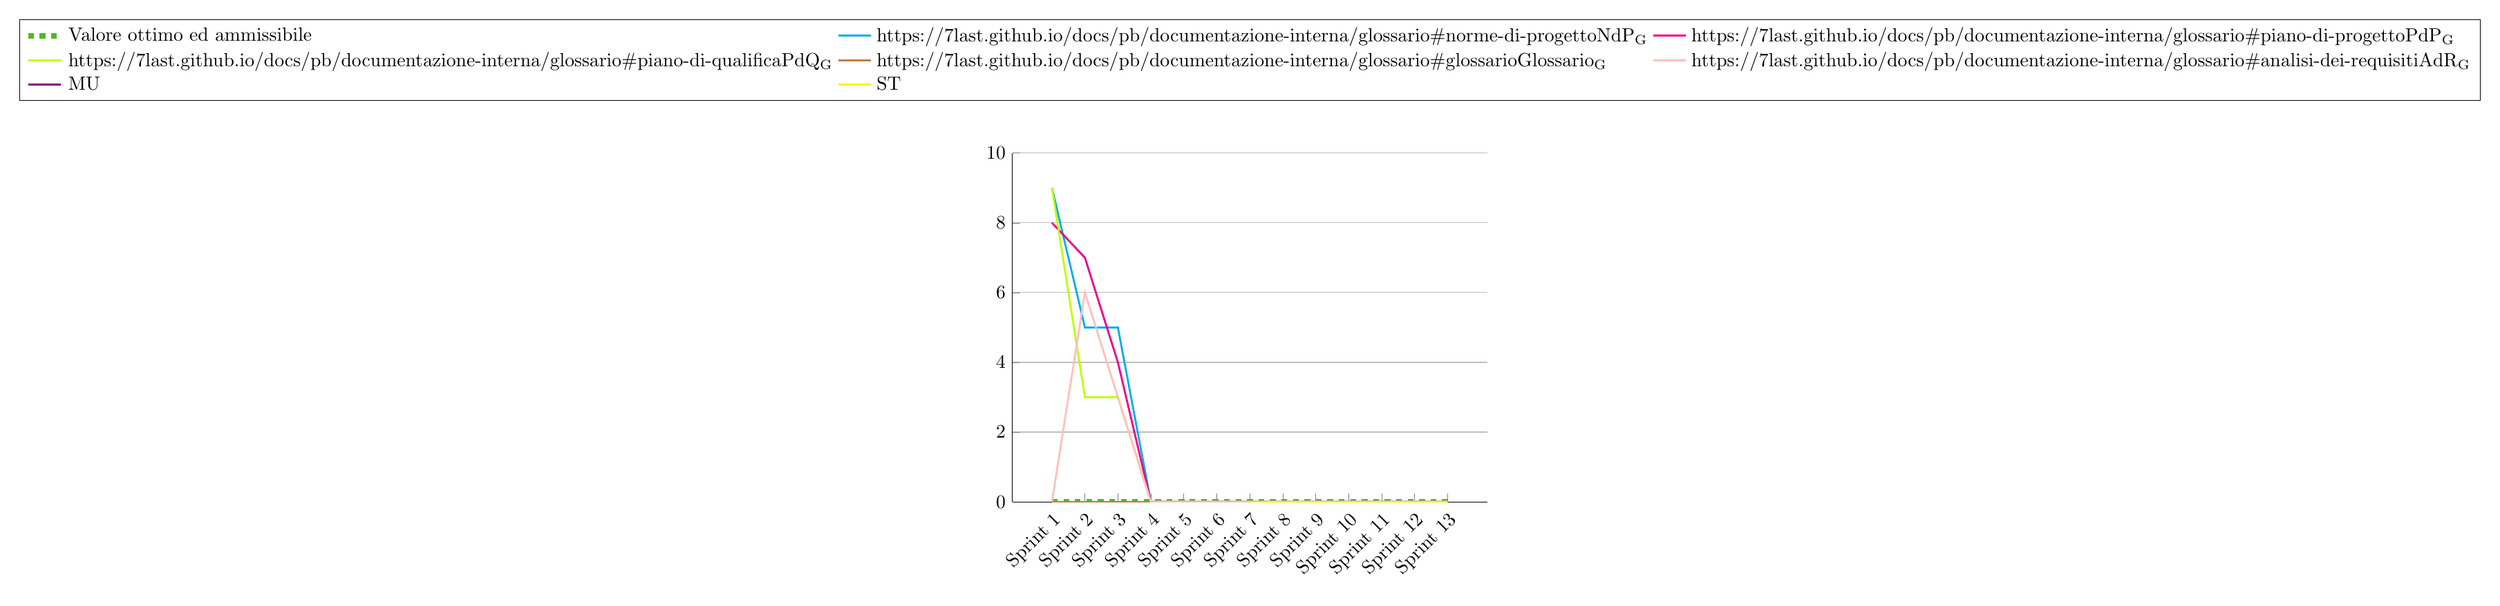
\begin{tikzpicture}
        \begin{axis}[
            width  = 0.85*\textwidth,
            height = 8cm,
            ymajorgrids = true,
            symbolic x coords={Sprint 1, Sprint 2, Sprint 3, Sprint 4, Sprint 5, Sprint 6, Sprint 7, Sprint 8, Sprint 9, Sprint 10, Sprint 11, Sprint 12, Sprint 13},
            xtick = data,
            ymin=0, ymax=10,
            axis lines*=left,
            legend cell align=left,
            legend style={
                at={(0.5,1.15)},
                anchor=south,
                column sep=0.1ex,
                legend columns=3
            },
            xticklabel style={rotate=45, anchor=north east, yshift=0ex, xshift=0ex}
        ]
            \addplot[color=opt, style={dashed, line width=3pt}, mark=none] coordinates { % ottimo e ammissibile = 0
                (Sprint 1, 0)
                (Sprint 2, 0)
                (Sprint 3, 0)
                (Sprint 4, 0)
                (Sprint 5, 0)
                (Sprint 6, 0)
                (Sprint 7, 0)
                (Sprint 8, 0)
                (Sprint 9, 0)
                (Sprint 10, 0)
                (Sprint 11, 0)
                (Sprint 12, 0)
                (Sprint 13, 0)
            };
            \addplot[color=cyan, style={line width=1pt}, mark=none] coordinates { % norme di progetto
                (Sprint 1, 9)
                (Sprint 2, 5)
                (Sprint 3, 5)
                (Sprint 4, 0)
                (Sprint 5, 0)
                (Sprint 6, 0)
                (Sprint 7, 0)
                (Sprint 8, 0)
                (Sprint 9, 0)
                (Sprint 10, 0)
                (Sprint 11, 0)
                (Sprint 12, 0)
                (Sprint 13, 0)
            };
            \addplot[color=magenta, style={line width=1pt}, mark=none] coordinates { % piano di progetto
                (Sprint 1, 8)
                (Sprint 2, 7)
                (Sprint 3, 4)
                (Sprint 4, 0)
                (Sprint 5, 0)
                (Sprint 6, 0)
                (Sprint 7, 0)
                (Sprint 8, 0)
                (Sprint 9, 0)
                (Sprint 10, 0)
                (Sprint 11, 0)
                (Sprint 12, 0)
                (Sprint 13, 0)
            };
            \addplot[color=lime, style={line width=1pt}, mark=none] coordinates { % piano di qualifica
                (Sprint 1, 9)
                (Sprint 2, 3)
                (Sprint 3, 3)
                (Sprint 4, 0)
                (Sprint 5, 0)
                (Sprint 6, 0)
                (Sprint 7, 0)
                (Sprint 8, 0)
                (Sprint 9, 0)
                (Sprint 10, 0)
                (Sprint 11, 0)
                (Sprint 12, 0)
                (Sprint 13, 0)
            };
            \addplot[color=brown, style={line width=1pt}, mark=none] coordinates { % glossario
                (Sprint 1, 0)
                (Sprint 2, 0)
                (Sprint 3, 0)
                (Sprint 4, 0)
                (Sprint 5, 0)
                (Sprint 6, 0)
                (Sprint 7, 0)
                (Sprint 8, 0)
                (Sprint 9, 0)
                (Sprint 10, 0)
                (Sprint 11, 0)
                (Sprint 12, 0)
                (Sprint 13, 0)
            };
            \addplot[color=pink, style={line width=1pt}, mark=none] coordinates { % analisi dei requisiti
                (Sprint 1, 0)
                (Sprint 2, 6)
                (Sprint 3, 3)
                (Sprint 4, 0)
                (Sprint 5, 0)
                (Sprint 6, 0)
                (Sprint 7, 0)
                (Sprint 8, 0)
                (Sprint 9, 0)
                (Sprint 10, 0)
                (Sprint 11, 0)
                (Sprint 12, 0)
                (Sprint 13, 0)
            };
            \addplot[color=violet, style={line width=1pt}, mark=none] coordinates { % manuale utente
                (Sprint 7, 0)
                (Sprint 8, 0)
                (Sprint 9, 0)
                (Sprint 10, 0)
                (Sprint 11, 0)
                (Sprint 12, 0)
                (Sprint 13, 0)
            };
            \addplot[color=yellow, style={line width=1pt}, mark=none] coordinates { % specifica tecnica
                (Sprint 7, 0)
                (Sprint 8, 0)
                (Sprint 9, 0)
                (Sprint 10, 0)
                (Sprint 11, 0)
                (Sprint 12, 0)
                (Sprint 13, 0)
            };
            \legend{Valore ottimo ed ammissibile, \href{https://7last.github.io/docs/pb/documentazione-interna/glossario\#norme-di-progetto}{NdP\textsubscript{G}}, \href{https://7last.github.io/docs/pb/documentazione-interna/glossario\#piano-di-progetto}{PdP\textsubscript{G}}, \href{https://7last.github.io/docs/pb/documentazione-interna/glossario\#piano-di-qualifica}{PdQ\textsubscript{G}}, \href{https://7last.github.io/docs/pb/documentazione-interna/glossario\#glossario}{Glossario\textsubscript{G}}, \href{https://7last.github.io/docs/pb/documentazione-interna/glossario\#analisi-dei-requisiti}{AdR\textsubscript{G}}, MU, ST}
        \end{axis}
    \end{tikzpicture}
    \caption{Errori ortografici per ciascun documento}
\end{figure*}
%--------- FINE GRAFICO -----------%
\begin{flushleft}
\textbf{RTB} \\
Si noti come inizialmente il numero di errori di ortografia rilevati nei documenti sia elevato, per poi diminuire progressivamente. Questo indica che il gruppo \textit{7Last} ha migliorato la qualità della documentazione prodotta, riducendo gli errori di ortografia. \\
\textbf{PB} \\
Come si può notare dal grafico a partire dal quarto sprint la documentazione prodotta non presenta più errori di ortografia. Questo è dovuto all'utilizzo di strumenti di controllo ortografico automatici in fase di \textit{merge} dei branch nel repository, gestiti mediante l'utilizzo delle \textit{GitHub Actions}. Questo ha permesso di impedire in modo sistematico l'inserimento di errori di ortografia nei documenti prodotti.
\end{flushleft}

\newpage
\subsection{Qualità del processo di gestione della qualità}
\subsubsection{25M-QMS - Metriche di qualità soddisfatte}
%--------- GRAFICO -----------%
\begin{figure*}[!h]
    \centering
    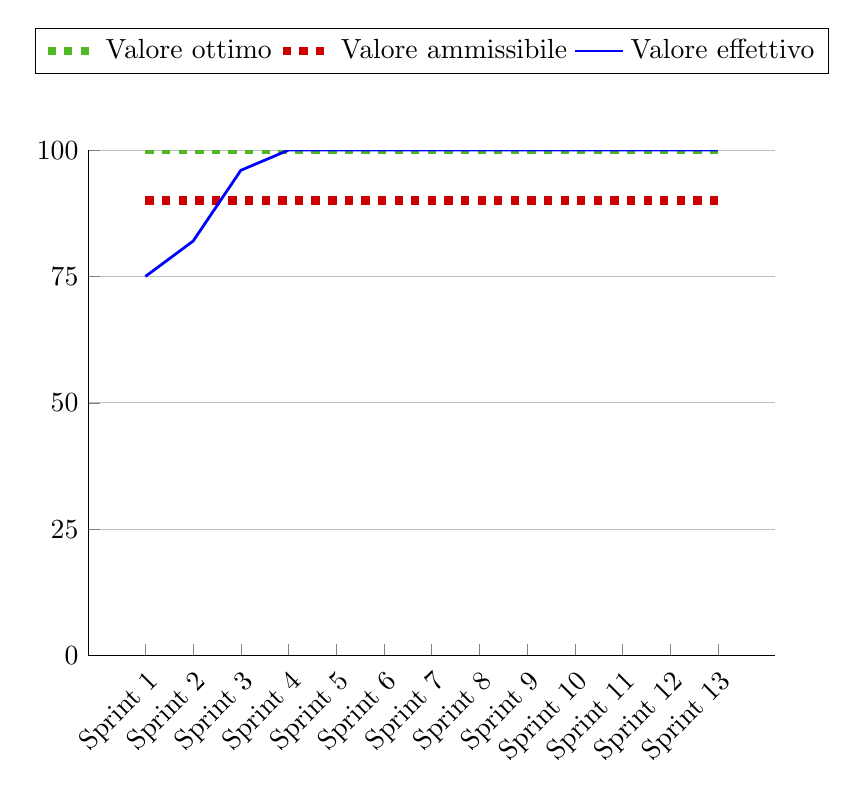
\begin{tikzpicture}
        \begin{axis}[
            width  = 0.85*\textwidth,
            height = 8cm,
            ymajorgrids = true,
            symbolic x coords={Sprint 1, Sprint 2, Sprint 3, Sprint 4, Sprint 5, Sprint 6, Sprint 7, Sprint 8, Sprint 9, Sprint 10, Sprint 11, Sprint 12, Sprint 13},
            xtick = data,
            ytick = {0, 25, 50, 75, 100},
            ymin=0, ymax=100,
            axis lines*=left,
            legend cell align=left,
            legend style={
                at={(0.5,1.15)},
                anchor=south,
                column sep=0.1ex,
                legend columns=3
            },
            xticklabel style={rotate=45, anchor=north east, yshift=0ex, xshift=0ex}
        ]
            \addplot[color=opt, style={dashed, line width=3pt}, mark=none] coordinates { % ottimo = 100
                (Sprint 1, 100)
                (Sprint 2, 100)
                (Sprint 3, 100)
                (Sprint 4, 100)
                (Sprint 5, 100)
                (Sprint 6, 100)
                (Sprint 7, 100)
                (Sprint 8, 100)
                (Sprint 9, 100)
                (Sprint 10, 100)
                (Sprint 11, 100)
                (Sprint 12, 100)
                (Sprint 13, 100)
            };
            \addplot[color=amm, style={dashed, line width=3pt}, mark=none] coordinates { % ammissibile = 90
                (Sprint 1, 90)
                (Sprint 2, 90)
                (Sprint 3, 90)
                (Sprint 4, 90)
                (Sprint 5, 90)
                (Sprint 6, 90)
                (Sprint 7, 90)
                (Sprint 8, 90)
                (Sprint 9, 90)
                (Sprint 10, 90)
                (Sprint 11, 90)
                (Sprint 12, 90)
                (Sprint 13, 90)
            };
            \addplot[color=blue, style={line width=1pt}, mark=none] coordinates {
                (Sprint 1, 75)
                (Sprint 2, 82)
                (Sprint 3, 96)
                (Sprint 4, 100)
                (Sprint 5, 100)
                (Sprint 6, 100)
                (Sprint 7, 100)
                (Sprint 8, 100)
                (Sprint 9, 100)
                (Sprint 10, 100)
                (Sprint 11, 100)
                (Sprint 12, 100)
                (Sprint 13, 100)
            };
            \legend{Valore ottimo, Valore ammissibile, Valore effettivo}
        \end{axis}
    \end{tikzpicture}
    \caption{Percentuale di metriche di qualità soddisfatte}
\end{figure*}
%--------- FINE GRAFICO -----------%
\begin{flushleft}
\textbf{RTB} \\
Osservando il grafico si può notare come inizialmente il valore delle metriche soddisfatte sia inferiore al valore ammissibile, questo è dovuto principalmente all'inesperienza del team. Successivamente l'andamento cresce progressivamente fino ad arrivare al 100\% nell'ultimo sprint. Questo indica un miglioramento progressivo del \textit{Way of Working} del gruppo. \\
\textbf{PB} \\
Come si evince dal grafico, il cruscotto di valutazione della qualità ha permesso al gruppo di monitorare costantemente il soddisfacimento delle metriche di qualità, ottenendo così un miglioramento progressivo fino al raggiungimento del 100\% delle metriche soddisfatte.
\end{flushleft}

\newpage
\subsection{Qualità del processo di verifica}
\subsubsection{26M-CC - Code coverage}
%--------- GRAFICO -----------%
\begin{figure*}[!h]
    \centering
    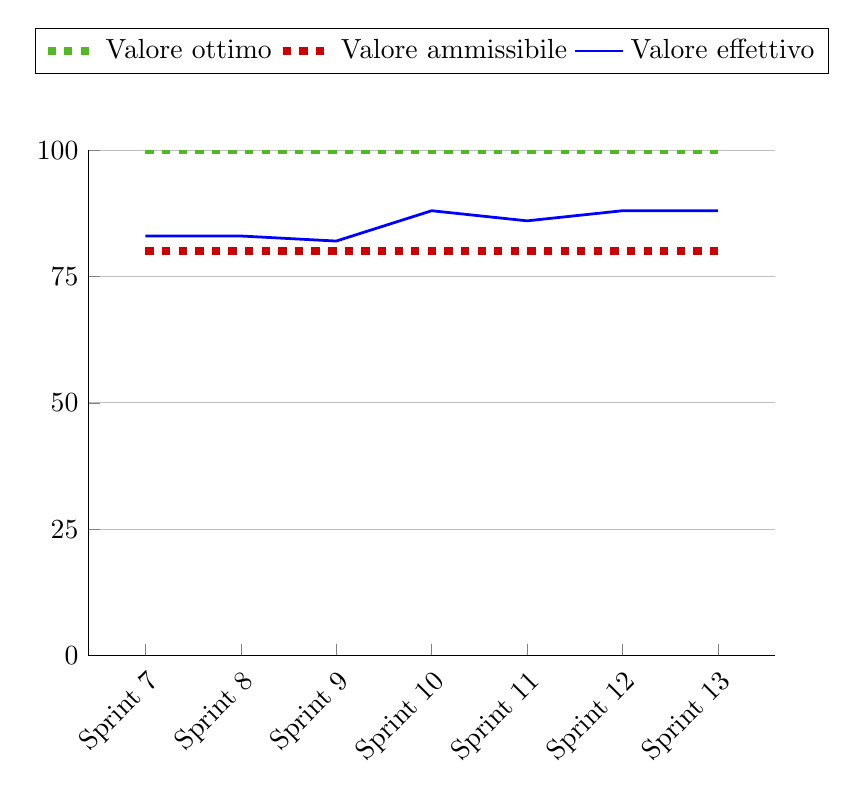
\begin{tikzpicture}
        \begin{axis}[
            width  = 0.85*\textwidth,
            height = 8cm,
            ymajorgrids = true,
            symbolic x coords={Sprint 7, Sprint 8, Sprint 9, Sprint 10, Sprint 11, Sprint 12, Sprint 13},
            xtick = data,
            ytick = {0, 25, 50, 75, 100},
            ymin=0, ymax=100,
            axis lines*=left,
            legend cell align=left,
            legend style={
                at={(0.5,1.15)},
                anchor=south,
                column sep=0.1ex,
                legend columns=-1
            },
            xticklabel style={rotate=45, anchor=north east, yshift=0ex, xshift=0ex}
            ]
            \addplot[color=opt, style={dashed, line width=3pt}, mark=none] coordinates {
                (Sprint 7, 100)
                (Sprint 8, 100)
                (Sprint 9, 100)
                (Sprint 10, 100)
                (Sprint 11, 100)
                (Sprint 12, 100)
                (Sprint 13, 100)
            };
            \addplot[color=amm, style={dashed, line width=3pt}, mark=none] coordinates {
                (Sprint 7, 80)
                (Sprint 8, 80)
                (Sprint 9, 80)
                (Sprint 10, 80)
                (Sprint 11, 80)
                (Sprint 12, 80)
                (Sprint 13, 80)
            };
            \addplot[color=blue, style={line width=1pt}, mark=none] coordinates {
                (Sprint 7, 83)
                (Sprint 8, 83)
                (Sprint 9, 82)
                (Sprint 10, 88)
                (Sprint 11, 86)
                (Sprint 12, 88)
                (Sprint 13, 88)
            };
            \legend{Valore ottimo, Valore ammissibile, Valore effettivo}
        \end{axis}
    \end{tikzpicture}
    \caption{Percentuale di code coverage dei test implementati}
\end{figure*}
%--------- FINE GRAFICO -----------% \\
\begin{flushleft}
\textbf{PB} \\
Al settimo sprint sono stati introdotti i primi test e fin da subito abbiamo voluto garantire la qualità del codice utilizzando le \textit{Github Actions} per impedire che venisse effettuato il \textit{merge} di codice non testato o che non superasse la percentuale minima prevista per ciascun test. Questo ha permesso di garantire un'alta percentuale di code coverage fin da subito, con un andamento costante e in crescita.
\end{flushleft}

\newpage
\subsubsection{27M-BC - Branch coverage}
%--------- GRAFICO -----------%
\begin{figure*}[!h]
    \centering
    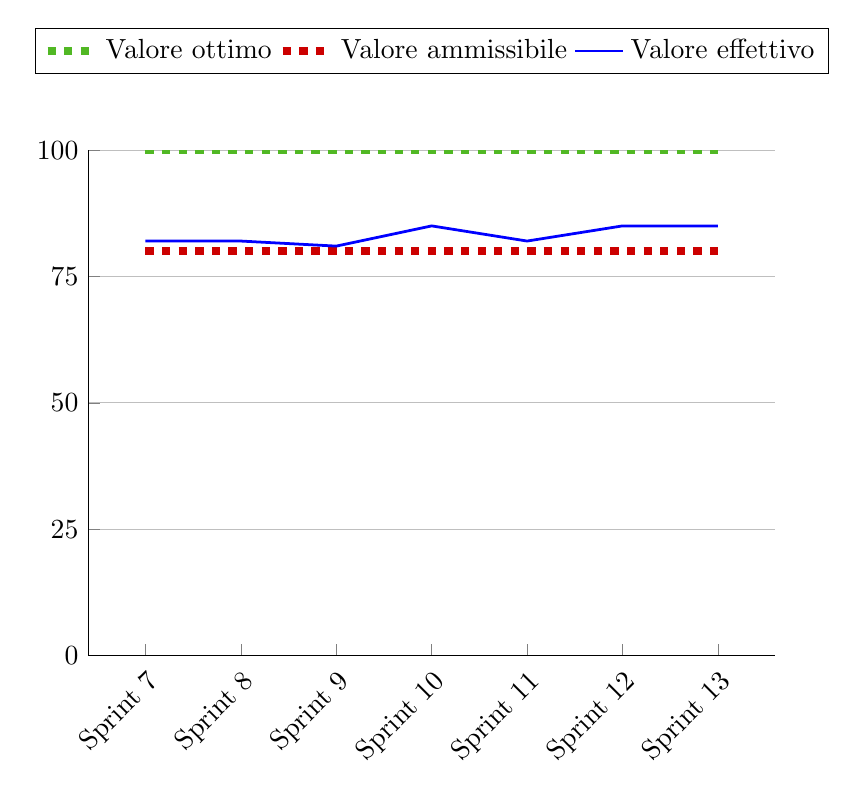
\begin{tikzpicture}
        \begin{axis}[
            width  = 0.85*\textwidth,
            height = 8cm,
            ymajorgrids = true,
            symbolic x coords={Sprint 7, Sprint 8, Sprint 9, Sprint 10, Sprint 11, Sprint 12, Sprint 13},
            xtick = data,
            ytick = {0, 25, 50, 75, 100},
            ymin=0, ymax=100,
            axis lines*=left,
            legend cell align=left,
            legend style={
                at={(0.5,1.15)},
                anchor=south,
                column sep=0.1ex,
                legend columns=3
            },
            xticklabel style={rotate=45, anchor=north east, yshift=0ex, xshift=0ex}
            ]
            \addplot[color=opt, style={dashed, line width=3pt}, mark=none] coordinates {
                (Sprint 7, 100)
                (Sprint 8, 100)
                (Sprint 9, 100)
                (Sprint 10, 100)
                (Sprint 11, 100)
                (Sprint 12, 100)
                (Sprint 13, 100)
            };
            \addplot[color=amm, style={dashed, line width=3pt}, mark=none] coordinates {
                (Sprint 7, 80)
                (Sprint 8, 80)
                (Sprint 9, 80)
                (Sprint 10, 80)
                (Sprint 11, 80)
                (Sprint 12, 80)
                (Sprint 13, 80)
            };
            \addplot[color=blue, style={line width=1pt}, mark=none] coordinates {
                (Sprint 7, 82)
                (Sprint 8, 82)
                (Sprint 9, 81)
                (Sprint 10, 85)
                (Sprint 11, 82)
                (Sprint 12, 85)
                (Sprint 13, 85)
            };
            \legend{Valore ottimo, Valore ammissibile, Valore effettivo}
        \end{axis}
    \end{tikzpicture}
    \caption{Percentuale di branch coverage dei test implementati}
\end{figure*}
%--------- FINE GRAFICO -----------% \\
\begin{flushleft}
\textbf{PB} \\
Anche in questo grafico si può notare come il gruppo \textit{7Last} abbia lavorato in modo costante per garantire la qualità del codice, con un'andamento costante e in crescita della percentuale di branch coverage. Come detto prima, questo è stato possibile grazie all'utilizzo delle \textit{GitHub Actions} per impedire il \textit{merge} di codice non testato o che non superasse la percentuale minima prevista per ciascun test.
\end{flushleft}

\newpage
\subsubsection{28M-SC - Statement coverage}
%--------- GRAFICO -----------%
\begin{figure*}[!h]
    \centering
    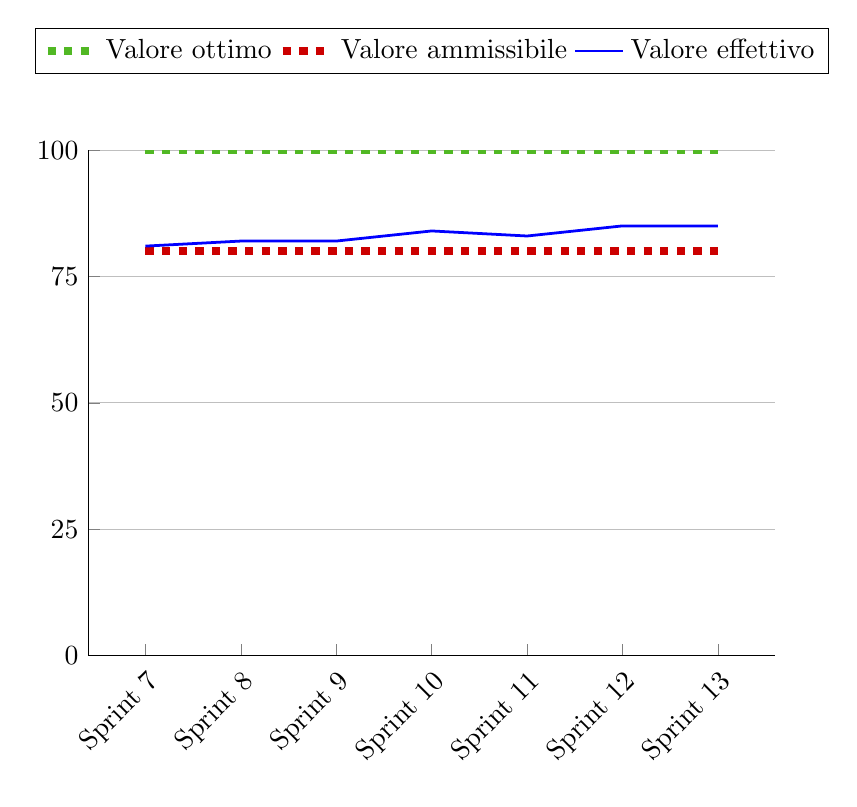
\begin{tikzpicture}
        \begin{axis}[
            width  = 0.85*\textwidth,
            height = 8cm,
            ymajorgrids = true,
            symbolic x coords={Sprint 7, Sprint 8, Sprint 9, Sprint 10, Sprint 11, Sprint 12, Sprint 13},
            xtick = data,
            ytick = {0, 25, 50, 75, 100},
            ymin=0, ymax=100,
            axis lines*=left,
            legend cell align=left,
            legend style={
                at={(0.5,1.15)},
                anchor=south,
                column sep=0.1ex,
                legend columns=3
            },
            xticklabel style={rotate=45, anchor=north east, yshift=0ex, xshift=0ex}
            ]
            \addplot[color=opt, style={dashed, line width=3pt}, mark=none] coordinates {
                (Sprint 7, 100)
                (Sprint 8, 100)
                (Sprint 9, 100)
                (Sprint 10, 100)
                (Sprint 11, 100)
                (Sprint 12, 100)
                (Sprint 13, 100)
            };
            \addplot[color=amm, style={dashed, line width=3pt}, mark=none] coordinates {
                (Sprint 7, 80)
                (Sprint 8, 80)
                (Sprint 9, 80)
                (Sprint 10, 80)
                (Sprint 11, 80)
                (Sprint 12, 80)
                (Sprint 13, 80)
            };
            \addplot[color=blue, style={line width=1pt}, mark=none] coordinates {
                (Sprint 7, 81)
                (Sprint 8, 82)
                (Sprint 9, 82) 
                (Sprint 10, 84)
                (Sprint 11, 83)
                (Sprint 12, 85)
                (Sprint 13, 85)
            };
            \legend{Valore ottimo, Valore ammissibile, Valore effettivo}
        \end{axis}
    \end{tikzpicture}
    \caption{Percentuale di statement coverage dei test implementati}
\end{figure*}
%--------- FINE GRAFICO -----------% \\
\begin{flushleft}
\textbf{PB} \\
Come già evidenziato in precedenza, anche qui abbiamo la conferma che il gruppo \textit{7Last} ha lavorato per garantire la qualità del codice, con un'andamento costante e in crescita della percentuale di statement coverage. Anche in questo caso, questo è stato possibile grazie all'utilizzo delle \textit{GitHub Actions} per impedire il \textit{merge} di codice non testato o che non superasse la percentuale minima prevista per ciascun test.
\end{flushleft}

\newpage
\subsubsection{29M-FD - Failure density}
%--------- GRAFICO -----------%
\begin{figure*}[!h]
    \centering
    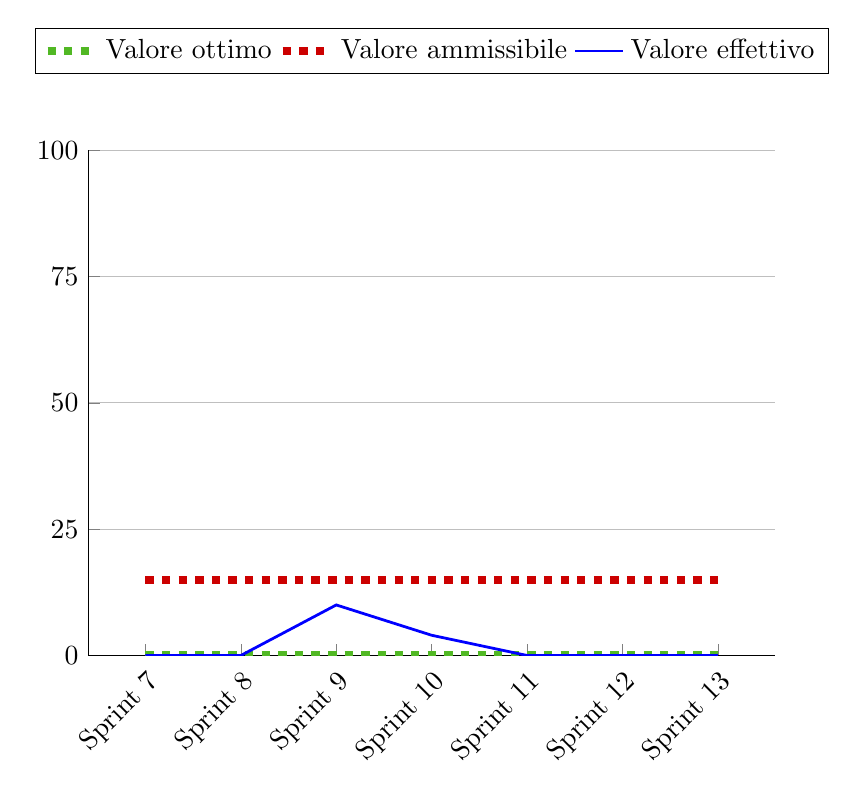
\begin{tikzpicture}
        \begin{axis}[
            width  = 0.85*\textwidth,
            height = 8cm,
            ymajorgrids = true,
            symbolic x coords={Sprint 7, Sprint 8, Sprint 9, Sprint 10, Sprint 11, Sprint 12, Sprint 13},
            xtick = data,
            ytick = {0, 25, 50, 75, 100},
            ymin=0, ymax=100,
            axis lines*=left,
            legend cell align=left,
            legend style={
                at={(0.5,1.15)},
                anchor=south,
                column sep=0.1ex,
                legend columns=3
            },
            xticklabel style={rotate=45, anchor=north east, yshift=0ex, xshift=0ex}
            ]
            \addplot[color=opt, style={dashed, line width=3pt}, mark=none] coordinates {
                (Sprint 7, 0)
                (Sprint 8, 0)
                (Sprint 9, 0)
                (Sprint 10, 0)
                (Sprint 11, 0)
                (Sprint 12, 0)
                (Sprint 13, 0)
            };
            \addplot[color=amm, style={dashed, line width=3pt}, mark=none] coordinates {
                (Sprint 7, 15)
                (Sprint 8, 15)
                (Sprint 9, 15)
                (Sprint 10, 15)
                (Sprint 11, 15)
                (Sprint 12, 15)
                (Sprint 13, 15)
            };
            \addplot[color=blue, style={line width=1pt}, mark=none] coordinates {
                (Sprint 7, 0)
                (Sprint 8, 0)
                (Sprint 9, 10)
                (Sprint 10, 4)
                (Sprint 11, 0)
                (Sprint 12, 0)
                (Sprint 13, 0)
            };
            \legend{Valore ottimo, Valore ammissibile, Valore effettivo}
        \end{axis}
    \end{tikzpicture}
    \caption{Percentuale di failure density}
\end{figure*}
%--------- FINE GRAFICO -----------% \\
\begin{flushleft}
\textbf{PB} \\
Dal grafico risultano evidenti i primi fallimenti rilevati in corrispondenza del nono sprint, naturale conseguenza dell'aggiunta di nuovi test che hanno permesso di rilevare errori non precedentemente individuati e correggerli. Successivamente si nota un calo dei fallimenti fino al raggiungimento del valore ottimo.
\end{flushleft}

\newpage
\subsubsection{30M-PTCP - Passed test case percentage}
%--------- GRAFICO -----------%
\begin{figure*}[!h]
    \centering
    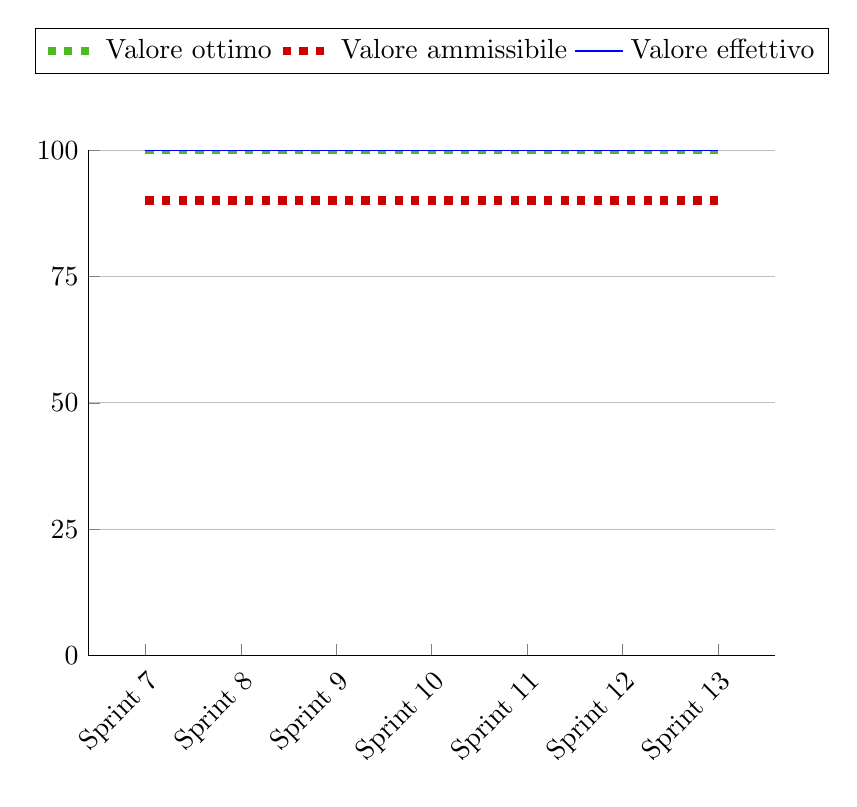
\begin{tikzpicture}
        \begin{axis}[
            width  = 0.85*\textwidth,
            height = 8cm,
            ymajorgrids = true,
            symbolic x coords={Sprint 7, Sprint 8, Sprint 9, Sprint 10, Sprint 11, Sprint 12, Sprint 13},
            xtick = data,
            ytick = {0, 25, 50, 75, 100},
            ymin=0, ymax=100,
            axis lines*=left,
            legend cell align=left,
            legend style={
                at={(0.5,1.15)},
                anchor=south,
                column sep=0.1ex,
                legend columns=3
            },
            xticklabel style={rotate=45, anchor=north east, yshift=0ex, xshift=0ex}
            ]
            \addplot[color=opt, style={dashed, line width=3pt}, mark=none] coordinates {
                (Sprint 7, 100)
                (Sprint 8, 100)
                (Sprint 9, 100)
                (Sprint 10, 100)
                (Sprint 11, 100)
                (Sprint 12, 100)
                (Sprint 13, 100)
            };
            \addplot[color=amm, style={dashed, line width=3pt}, mark=none] coordinates {
                (Sprint 7, 90)
                (Sprint 8, 90)
                (Sprint 9, 90)
                (Sprint 10, 90)
                (Sprint 11, 90)
                (Sprint 12, 90)
                (Sprint 13, 90)
            };
            \addplot[color=blue, style={line width=1pt}, mark=none] coordinates {
                (Sprint 7, 100)
                (Sprint 8, 100)
                (Sprint 9, 100)
                (Sprint 10, 100)
                (Sprint 11, 100)
                (Sprint 12, 100)
                (Sprint 13, 100)
            };
            \legend{Valore ottimo, Valore ammissibile, Valore effettivo}
        \end{axis}
    \end{tikzpicture}
    \caption{Percentuale di casi di test superati}
\end{figure*}
%--------- FINE GRAFICO -----------% \\
\begin{flushleft}
\textbf{PB} \\
Grazie all'utilizzo delle \textit{GitHub Actions}, il gruppo \textit{7Last} è riuscito a garantire che tutti i test implementati venissero superati, con un'andamento costante fisso al 100\% già dall'implementazione dei primi test in corrispondenza del settimo sprint fino alla fine del progetto.
\end{flushleft}

\newpage
\subsection{Qualità del processo di gestione dei rischi}
\subsubsection{32M-NCR - Rischi non calcolati}
%--------- GRAFICO -----------%
\begin{figure*}[!h]
    \centering
    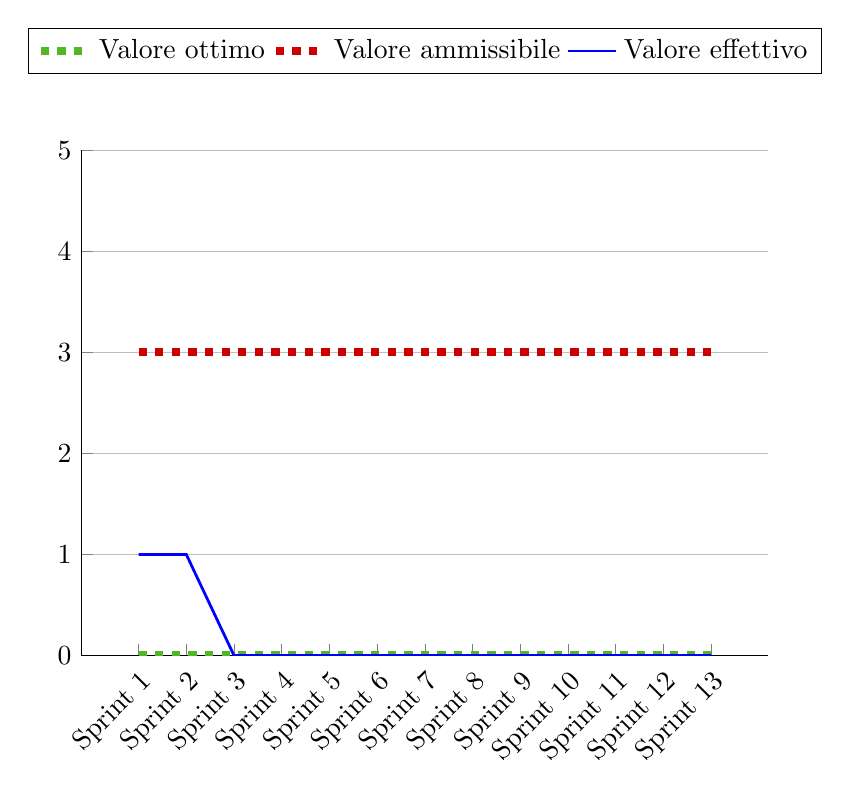
\begin{tikzpicture}
        \begin{axis}[
            width  = 0.85*\textwidth,
            height = 8cm,
            ymajorgrids = true,
            symbolic x coords={Sprint 1, Sprint 2, Sprint 3, Sprint 4, Sprint 5, Sprint 6, Sprint 7, Sprint 8, Sprint 9, Sprint 10, Sprint 11, Sprint 12, Sprint 13},
            xtick = data,
            ymin=0, ymax=5,
            axis lines*=left,
            legend cell align=left,
            legend style={
                at={(0.5,1.15)},
                anchor=south,
                column sep=0.1ex,
                legend columns=3
            },
            xticklabel style={rotate=45, anchor=north east, yshift=0ex, xshift=0ex}
        ]
            \addplot[color=opt, style={dashed, line width=3pt}, mark=none] coordinates { % ottimo = 0
                (Sprint 1, 0)
                (Sprint 2, 0)
                (Sprint 3, 0)
                (Sprint 4, 0)
                (Sprint 5, 0)
                (Sprint 6, 0)
                (Sprint 7, 0)
                (Sprint 8, 0)
                (Sprint 9, 0)
                (Sprint 10, 0)
                (Sprint 11, 0)
                (Sprint 12, 0)
                (Sprint 13, 0)
            };
            \addplot[color=amm, style={dashed, line width=3pt}, mark=none] coordinates { % ammissibile = 3
                (Sprint 1, 3)
                (Sprint 2, 3)
                (Sprint 3, 3)
                (Sprint 4, 3)
                (Sprint 5, 3)
                (Sprint 6, 3)
                (Sprint 7, 3)
                (Sprint 8, 3)
                (Sprint 9, 3)
                (Sprint 10, 3)
                (Sprint 11, 3)
                (Sprint 12, 3)
                (Sprint 13, 3)
            };
            \addplot[color=blue, style={line width=1pt}, mark=none] coordinates { % rischi non calcolati
                (Sprint 1, 1)
                (Sprint 2, 1)
                (Sprint 3, 0)
                (Sprint 4, 0)
                (Sprint 5, 0)
                (Sprint 6, 0)
                (Sprint 7, 0)
                (Sprint 8, 0)
                (Sprint 9, 0)
                (Sprint 10, 0)
                (Sprint 11, 0)
                (Sprint 12, 0)
                (Sprint 13, 0)
            };
            \legend{Valore ottimo, Valore ammissibile, Valore effettivo}
        \end{axis}
    \end{tikzpicture}
    \caption{Rischi non calcolati occorsi durante il progetto}
\end{figure*}
%--------- FINE GRAFICO -----------%
\begin{flushleft}
\textbf{RTB} \\
Dal grafico si evince che durante i primi sprint sono emersi rischi non calcolati, sintomo di una pianificazione non ottimale dovuta all'inesperienza. Successivamente il team ha accumulato esperienza, mediante automiglioramento, imparando a gestire e prevenire i rischi in modo migliore. \\
\textbf{PB} \\
Nella seconda parte del progetto non sono stati riscontrati rischi non calcolati, questo è dovuto all'esperienza acquisita dal gruppo \textit{7Last} che ha permesso di prevedere e gestire in modo efficace i rischi, evitando che si verificassero.
\end{flushleft}

\newpage
\subsection{Qualità del processo di pianificazione}
\subsubsection{33M-RSI - Requirements stability index}
%--------- GRAFICO -----------%
\begin{figure*}[!h]
    \centering
    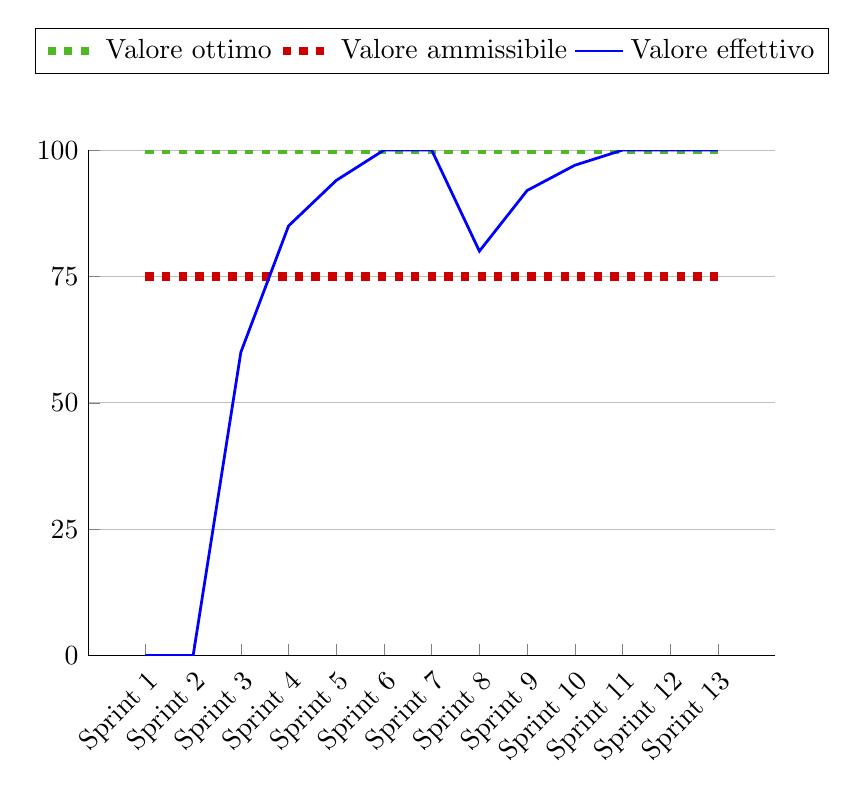
\begin{tikzpicture}
        \begin{axis}[
            width  = 0.85*\textwidth,
            height = 8cm,
            ymajorgrids = true,
            symbolic x coords={Sprint 1, Sprint 2, Sprint 3, Sprint 4, Sprint 5, Sprint 6, Sprint 7, Sprint 8, Sprint 9, Sprint 10, Sprint 11, Sprint 12, Sprint 13},
            xtick = data,
            ytick = {0, 25, 50, 75, 100},
            ymin=0, ymax=100,
            axis lines*=left,
            legend cell align=left,
            legend style={
                at={(0.5,1.15)},
                anchor=south,
                column sep=0.1ex,
                legend columns=3
            },
            xticklabel style={rotate=45, anchor=north east, yshift=0ex, xshift=0ex}
        ]
            \addplot[color=opt, style={dashed, line width=3pt}, mark=none] coordinates { % ottimo = 100
                (Sprint 1, 100)
                (Sprint 2, 100)
                (Sprint 3, 100)
                (Sprint 4, 100)
                (Sprint 5, 100)
                (Sprint 6, 100)
                (Sprint 7, 100)
                (Sprint 8, 100)
                (Sprint 9, 100)
                (Sprint 10, 100)
                (Sprint 11, 100)
                (Sprint 12, 100)
                (Sprint 13, 100)
            };
            \addplot[color=amm, style={dashed, line width=3pt}, mark=none] coordinates { % ammissibile = 75
                (Sprint 1, 75)
                (Sprint 2, 75)
                (Sprint 3, 75)
                (Sprint 4, 75)
                (Sprint 5, 75)
                (Sprint 6, 75)
                (Sprint 7, 75)
                (Sprint 8, 75)
                (Sprint 9, 75)
                (Sprint 10, 75)
                (Sprint 11, 75)
                (Sprint 12, 75)
                (Sprint 13, 75)
            };
            \addplot[color=blue, style={line width=1pt}, mark=none] coordinates { % RSI
                (Sprint 1, 0)
                (Sprint 2, 0)
                (Sprint 3, 60)
                (Sprint 4, 85)
                (Sprint 5, 94)
                (Sprint 6, 100)
                (Sprint 7, 100)
                (Sprint 8, 80)
                (Sprint 9, 92)
                (Sprint 10, 97)
                (Sprint 11, 100)
                (Sprint 12, 100)
                (Sprint 13, 100)
            };
            \legend{Valore ottimo, Valore ammissibile, Valore effettivo}
        \end{axis}
    \end{tikzpicture}
    \caption{Percentuale di stabilità dei requisiti}
\end{figure*}
%--------- FINE GRAFICO -----------%
\begin{flushleft}
\textbf{RTB} \\
L'analisi del RSI mostra un forte incremento tra il secondo e il terzo sprint, segnalando un'intensa attività di revisione e aggiustamento dei requisiti. Nei due sprint successivi, il RSI si stabilizza, indicando una riduzione delle modifiche e una maggiore stabilità dei requisiti. Questo andamento riflette un'efficace fase iniziale di consolidamento dei requisiti seguita da una stabilizzazione che facilita l'implementazione del progetto. \\
\textbf{PB} \\
Dal grafico si può notare come i requisiti abbiano subito alcune modifiche in corrispondenza dell'ottavo sprint (e successivi). Questo è dovuto alla necessità di apportare alcune modifiche ai requisiti in seguito ai consigli ricevuti dal professor Cardin durante la revisione RTB, oltre ad alcune variazioni concordate con il proponente su alcune funzionalità del prodotto. Questo ha permesso di migliorare la qualità del prodotto e di garantire una maggiore soddisfazione del proponente.
\end{flushleft}
